% This file is iccc.tex.  It contains the formatting instructions for and acts as a template for submissions to ICCC.  It borrows liberally from the AAAI and IJCAI formats and instructions.  It uses the files iccc.sty, iccc.bst and iccc.bib, the first two of which also borrow liberally from the same sources.

\documentclass[letterpaper]{article}
\usepackage{iccc}

\usepackage{graphicx}
\usepackage{times}
\usepackage{helvet}
\usepackage{courier}
\pdfinfo{
	/Title (Anything2vec: generalizing word2vec via the use of meaningful contexts)
	/Subject (Proceedings of ICCC)
	/Author (ICCC)}
% The file iccc.sty is the style file for ICCC proceedings.
%

%\title{Anything2vec: generalizing word2vec via the use of meaningful
%	contexts}
% Add something about its application to trope description - JJ 
%\author{Dan Ventura\\
%Computer Science Department\\
%Brigham Young University\\
%Provo, UT 84602  USA\\
%ventura@cs.byu.edu\\
%}
\setcounter{secnumdepth}{0}

\begin{document} 
	% \maketitle
	\begin{abstract}
		\begin{quote}
			% From the old paper:
			%   Word2vec has been a very successful algorithm that is able to give a
			% semantic representation to words on a corpus based in the context
			% they appear. In this paper we will try to extend this concept to
			% other {\em unordered} contexts. We will try to define this context
			% for movie (and TV) tropes.
			In this paper we present a generalized approach to extend the use of word2vec for non-traditional NLP (Natural Language Processing). In order to exemplify the idea, we use tvtropes dataset (trope names and film names only) to create a text corpus in order to give contextual information to any piece of data.
		\end{quote}
	\end{abstract}
	
	% From the old paper:
	% What are tropes and why we are interested
	
	% We need to find an embedding for tropes that allows us to do trope arithmetic and also process them, and movies in which they are used, in an uniform way.
	
	% We propose trope2vec
	
	% We analyse how it allows to explore the trope space and find
	% similarities between them.
	
	\section{Introduction}
	
	% Some help from: https://www.nature.com/scitable/topicpage/scientific-papers-13815490/
	
	% First, provide some context to orient those readers who are less familiar with your topic and to establish the importance of your work.

    % With growing diversity in personal food preference and regional cuisine style, personalized information systems that can transform a recipe into any selected regional cuisine style that a user might prefer would help food companies and professional chefs create new recipes.
    
 
    When we want to work with vector representations of words, word2vec is one of the most used algorithms since its appearance \cite{mikolov2013}.
    The vector obtained for each word has the ability to save memory of its environment. This vector is called embedding vector.
    Another interesting feature of embeddings vectors is that it is possible to perform concept arithmetic. For example, it would be possible to subtract and add vectors so that we obtain another vector resulting from the operation: Paris - France + Italy = Rome. However, in order to apply this algorithm, it is necessary to have a sufficiently large corpus written in natural language. Some examples of these frequently used corpus are Wikipedia or Google News dumps, usually greather than one GB of plain text. \\
    
    But, it would be possible to apply word2vec to non natural language corpus? With this work we want to demonstrate that it is possible to obtain embeddings vectors using word2vec of an artificially created corpus. To demonstrate this idea we will use data from films and tropes obtained from tvtropes.org website. Tv Tropes is a collaborative website created in 2004 to share information about tips, narrative or cinematographic techniques used in creative works such as movies, tv series or books. Each film, TV series or other
    fiction element usually includes a description and a list of associated
    tropes. Tropes pages usually contains a description followed by a list
    of films or a narrative resource that uses this trope.\\
    
	% Second, state the need for your work, as an opposition between what the scientific community currently has and what it wants.
	
	Obtaining a vector representation of concepts is an old problem that can be solved in different ways. Some of these solutions use only word coding without considering the context. This type of representation has a more limited use. Other works like \cite{kazama2018} have shown that it is
	possible to use word2vec to obtain vectors from non-NLP information
	sources. Our approach is based on the use of the fundamental elements
	of information (in our case the tropes) to generate an artificial
	narrative or corpus that can give a similar meaning to the concepts
	that they would have in a text written by humans. This artificially
	created text should represent the relationships between entities in
	the same way that a human would relate them in a descriptive text
	about these entities. If the artificial corpus is correctly
	constructed, it should produce some embedding vectors with the
	capacity to offer us a correct arithmetic of concepts. 
	
	We want the word representation to have the following characteristics: 
	
	\begin{itemize}

	\item That includes the context of the trope
	\item relatively compact
	\item capable of doing arithmetic
	\item uniform for tropes and movies.
		
    \end{itemize}
	   
    % I need help to write this part   
	   
	% Third, indicate what you have done in an effort to address the need (this is the task).

    In order to solve the problem, we have downloaded films data from word2vec. Then we have extracted a subset of films whose number of tropes is less than a certain thresold. From this subset of films and tropes, we have built an artificial corpus on which to apply the word2vec algorithm and generate embeddings. To evaluate that the subset of tropes is representative, we have verified that 92\% of the subset are among the most frequently used tropes. With the obtained vectors we have generated a classification to verify correspondence between embeddings and real films-tropes relationships. From the vectors that represent the tropes we have created a vector for the film. As a result, we have verified that the artificially generated corpus fulfills the desired objective. Obtained graphic representation shows that obtained clusters are correlated with real relationships observed between tropes and between tropes and films.\\
 
 % How we want to solve that problem: we think that an adaptation of word2vec should be possible
 % This is what you say above - JJ	
		% How we do it:
	% * Methodology for creating the context of every trope
	% * Methodology for representing movies using trope vector
	% * How we evaluate the goodness of the set of movies/tropes chosen.
	
	% Our results
	% * Clustering
	% * Graph representation
	% * Movie representation
	% * Example of synthetic movie generation.
	
	
	% Finally, preview the remainder of the paper to mentally prepare readers for its structure, in the object of the document.

	The rest of the paper is organized as follows. Next we present the
	state of the art in using embedding for problems other than language
	processing, as well as an overview of the use of tropes for narrative
	generation. The methodology is presented next in Section
	\ref{sec:met}, with results presented in Section \ref{sec:res}
	followed by the conclusion that closes the paper.
	
	
	\section{State of the art}
	
	Unlike systems such as MovieLens \cite{10.1145/2827872}, which focus
	on recommendation, our ultimate
	interest in representing movie tropes lies in the possibility of
	generating narratives \cite{10.5555/931357} that are optimal from some point of view (mainly
	coherence) from a set of tropes. Out of all the possible methods to
	generate narratives \cite{van2019narrative} this is one that has
	probably been explored the least; Sullivan et
	al. \cite{10.1145/3235765.3235819} used tropes in the tarot deck to
	generate narratives via combinations, but other than that, in general
	the presence of tropes has been used more for evaluation of generated
	narratives \cite{gervas2012story} that as part of the generation
	itself; in general, tropes are understood as constraints for
	characters or plots \cite{Thompson18NarrativeEvents}, but, of course,
	there are many kind of tropes and some of them can be converted
	directly into plots; for instance, {\sf AgeStereotypicalFood} informs
	of the fact that eating or talking about food will be introduced into
	the narrative.
	
	This work has been inspired by other that have used
	word2vec-like embeddings for purposes that are totally
	unrelated to natural language; a good survey is presented in
	\cite{nonnlp19}. In general, creating embeddings out of data
	is done with several purposes: reducing dimensionality, but
	also trying to create a data representation with semantics; as
	a side effect, this data representation will enable ``content
	arithmetics''. In our previous work
	\cite{doi:10.1111/exsy.12525} we used a direct representation
	of tropes; every dimension in a vector represented a trope,
	once less frequent ones had been excluded. However, this left
	out many possibly meaningful tropes, and still the size of the
	vectors was huge, representing its own challenge when using
	them in a deep learning algorithm.
	
	This was one of the intentions of Kazama et al. in
	\cite{kazama2018}, which is actually the paper that inspired
	our work. The content they wanted to represent was the concept
	of ``regional cuisine'', so that a regional cuisine embedding
	could be added or substracted from the embedding of a dish to
	create a new, equivalent one in that new regional
	environment. The kind of data they were working with is
	similar to the one we use in this paper: dish ingredients. As
	in our case, there's no natural order in the ingredients, but
	unlike our case, the amount of ingredients that are used in a
	dish are really limited, at least if you exclude
	seasoning. But they achieved their objective: being able to do
	recipe arithmetics, but also create meaningful maps of food
	that can be used in deep learning or any other environment.
	
	Most other applications are similar, in a way, to this one,
	and most of them are also recent. There was a publication in
	the Twitter engineering blog \cite{twitter:embeddings},
	apparently pointing to their use studying the social networks
	of users. Initial work was done by Grbovic et al. applied it to product recommendation
	\cite{Grbovic2015}, Vasile et al. applied it to product
	recommendation systems \cite{vasile2016} while McAuley et
	al. \cite{DBLP:journals/corr/McAuleyPL15} used embedding
	arithmetics to find complementary products to others that had
	been already purchased; these articles were
	probably ones of the first to use this kind of
	representation.
	
	Word embeddings to create clustering, however, go back at
	least to Kohonen's work in the 90s
	\cite{kohonen1997exploration}, which tried to create
	embeddings by assigning a word a vector created from averaging
	randomly created vectors initially assigned to its neighboring
	vectors. This work was extended to ant clustering algorithms
	to create word clusterings by Ramos et
	al. \cite{DBLP:journals/corr/abs-cs-0412075}.
	
	The fact that the variety of data embeddings have been applied
	to, as well as the kind of applications created with is so
	wide, has encouraged us to apply it to the study of movies via
	their tropes, as well as its eventual optimization.
	
	\section{Methodology}
	\label{sec:met}
	
	In order to obtain a vector representation of concepts from an artificially generated corpus we have followed the following steps:
	
	\begin{enumerate}
		\item Download film information from tvtropes.org and their associated tropes
		\item Select films with number of tropes less than a certain thresold
		\item After this, we create phrases from permutations of the tropes associated with each movie
		\item Build word2vec model. After that we will have a numerical vector for each trope.\\
		\item Visualize tropes vector space in order to detect clusters and possible data organization. \item Create a Vector for each film as the sumatory of all tropes vectors. \\

    \end{enumerate}

	% Main idea here is that the artificial corpus will represent the true as much as possible. ¿how we can achieve that?
	% We need a parameter that let us reinforce more real relationships between elements that are stronger. For example, in case of films,
	% we can use a value of film popularity to write more times in corpus information about a blockbuster film. We have to do the same with 
	% es like tropes. More relevant tropes will be them who appear more times in films, so these tropes have to appear more times in 
	% corpus. Ideal situation will be that artificial corpus emulate real conextions faithfully.\\
	% Let's use imdb blockbuster films sort by votes. Votes will be the number to reinforce more in corpus films that have more votes.	 
	% we can apply an incremental approach to do that, creating verification check lists to see if certain part of the corpus fits reality. 
	% for next paper version
	
	
	
	

To obtain this artificial corpus, we place together entities
that are connected. In the example of tvtropes, we will
generate the artificial corpus generating phrases that put
together film tropes. In order to generate the corpus, we will
select films that have a maximum of 15 tropes. We take this
initial limit since we will generate all the variations
without repetitions of 15 elements taken in groups of n
elements. his method can give us enough size corpus to train
the model using word2vec algorithm.
In order to generate the artificial corpus, we have followed this procedure. We have selected those films that have a maximum of MAX\_TROPES and eliminating those that have zero or 1 trope.   

    \subsection{Creating artificial corpus}
		
	\begin{table}[t]
		\centering
		\begin{tabular}{|p{0.20\linewidth}|p{0.2\linewidth}|p{0.2\linewidth}|p{0.2\linewidth}|}
			\hline
			\textbf{(MaxTrop, NgramSize)}& \textbf{(16,9)} & \textbf{(15, 9)} & \textbf{(12,7)}\\
			\hline
			\hline
			Tropes Subset Size&8125&7383& 5500\\
			\hline
			Film Subset Size&2686&2380& 1674\\
			\hline
			Corpus File Size (MB)&747&264& 32\\
			\hline
			Word2vec Model file Size(MB)&5.6&4.9&4.9\\
			\hline
			Vocab Size& 7078 & 6173 & 4653\\
			\hline
			Words in train file& 48893099 &17386514&2056372\\
			\hline

		\end{tabular}
		\caption{Characteristics of different corpus sizes and word2vec models created by varying MAX\_TROPES and NGRAM\_SIZE (word2vec argument min-count = 5). Execution time for i7 5500u 2.40 Ghz 16GB RAM}
		\label{tab:corpusSize}
	\end{table}
	
	This filtering process generates a reduced set of tropes. Table \ref{tab:corpusSize} shows characteristics of different sets of films, tropes and generated corpus. Full set of tropes have 25405 different tropes. Figure \ref{fig:tropesdistributionasociatedtofilms} shows the accumulative distribution of tropes and films, where 250 threshold will include more than 25000 tropes. In case of subset of films with number of tropes between 15 and 2 tropes has only 6524 different tropes. 
	It is important to check if our subset of tropes is relevant within the total set of tropes. To do so, we order the tropes by number of times it appears in a movie. In case of subset of tropes from films between 15 and 2 tropes, our subset covers the 99,2 percent of the 250 most popular tropes, so we can consider it a representative subset. 
	
	Tvtropes dataset has 673258 pairs film-trope. 73917 duplicate values in pairs. After apply word2vect to artificially created corpus, a set of embedding vectors will be created. The embedding vector integrate information about the context of a certain word and it is easy to find the relationships with other terms in corpus.\\
	To obtain this artificial corpus, we place together entities that are connected. In the example of tvtropes, we create the artificial corpus generating phrases that put together tropes used in a film. In order to generate the corpus, we will select films that have MAX\_TROPES tropes. We take this initial limit since we will generate all the variations without repetitions of MAX\_TROPES elements taken in groups of NGRAM\_SIZE elements. This method can give us a corpus with hundreds of Mega Bytes to train the model using word2vec algorithm. \\
	
	\begin{figure}
		\centering
		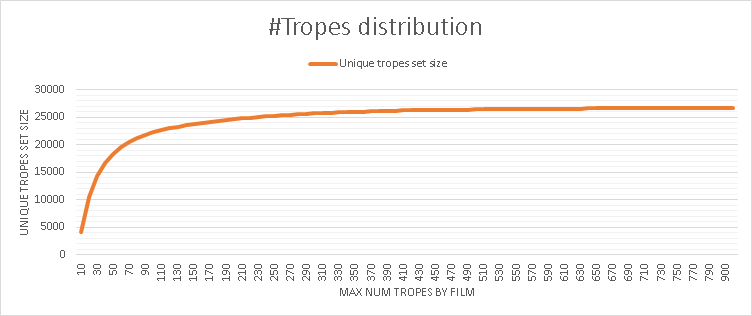
\includegraphics[width=1\linewidth]{../images/tropes_distribution_chart.png}
		\caption{Accumulative distribution of tropes associated to films}
		\label{fig:tropesdistributionasociatedtofilms}
	\end{figure}
	
	The challenge now is how to create a corpus that will be useful to find relationships between tropes and films. Each film has a description and a list of tropes, and each trope have a description and a list of films that uses this trope. Initially our dataset obtained from tvtropes.org 13th December 2019 included 12360 films and 26742 different tropes (25405 after remove duplicates). The film with higher number of tropes has 1028 tropes and the film with minimum number of tropes has 0 tropes. Tvtropes dataset has 673258 pairs film-trope. 73917 duplicate values in pairs. After apply word2vect to artificially created corpus, a set of embedding vectors will be created. The embedding vector integrate information about the context of a certain word and it is easy to find the relationships with other terms in corpus.\\
	
	The size of the corpus of variations without repetition of 15 tropes taken from 9 in 9 is 288 Mbytes. 9-size phrases have been created by making variations without repetition and ordering the result randomly \\
	
	\begin{center}
		
		${v}_{m,n} = m.(m-1).(m-2)...(m-n+1)$
		${v}_{15,9} = 1816214400$
		
	\end{center}
	
	%       % This kind of thing does not belong in a paper 
	%     Following line represent word2vec train parameters:\\
	% \begin{verbatim}
	% /word2vec 
	% -train ngrams_15_taken_9.txt 
	% -output ngrams_15_taken_9.bin 
	% -cbow 1 -size 200 -window 8 
	% -negative 25 -hs 0 
	% -sample 1e-4 -threads 20 
	% -binary 1 -iter 15
	% \end{verbatim}
	
	% There's no need to say what to do; focus on the results and the
	% methodology. Mechanical steps can be explained in the repository.
	
	\subsection{Building embedding vectors model}
	
	After that we will have a numerical vector for each trope.
	
	Once we have obtained the file with the corpus for training, using the word2vec package https://github.com/tmikolov/word2vec created by
	\cite{mikolov2013} we run word2vec program to obtain trained model. This model will help us to obtain a embedding vector associated to each trope.
	In our case, the corpus does not contain stop-words and other words lacking information. For this reason, we have performed different tests with
	word2vec by modifying the MIN\_COUNT parameter that eliminates words that appear less than MIN\_COUNT times. Table \ref{tab:variations-with-min-count-argument-15-9}
	shows different details of the model and its creation process by varying the argument mentioned above.
	We have detected that the same trope can be written in different ways. The way to separate the words that appear in the name of the trope is to write
	the first letter in uppercase. We have found that sometimes for the same trope the sequence of characters in upper and lower case is not the same. 
	In order to prevent the same trope from being taken as a different word, we have made a filter to convert trope names to lowercase.
	
	
	\begin{table}[t]
		\centering
		\begin{tabular}{|p{0.20\linewidth}|p{0.2\linewidth}|p{0.2\linewidth}|p{0.2\linewidth}|}
			\hline
			\textbf{(MaxTrop, NgramSize, Min Count)}& \textbf{(15, 9, 1)} & \textbf{(15,9, 3)} & \textbf{(15, 9, 5)}\\
			\hline
			\hline
			Vocab Size& 7384 & 6197 & 6173 \\
			\hline
			Words in train file& 17387907 & 17386591 & 17386514 \\
			\hline 
			
		\end{tabular}
		\caption{Characteristics of different word2vec models created by varying the MIN\_COUNT argument}
		\label{tab:variations-with-min-count-argument-15-9}
	\end{table}	
	
	\subsection{Visualize tropes vector}
	
	Visualize tropes vector space in order to detect clusters and possible data organization. \\
	In order to verify that the model built with word2vec fulfills its purpose, we need to perform different checks. On the one hand, 
	we must verify that the relations established between tropes of the model correspond to reality. 
	Visualizing relationships between tropes in generated model can help us to verify the goodness of the model.
	Therefore, the next task will be to generate a file with the numerical vector associated with each trope. 
	To generate this file, we have used a script that uses Gensim, an Open Source python library that include functions to manipulate
	word2vec bin files.
	Table \ref{tab:200dims-vectors-associated-to-tropes} shows the results in the number of tropes associated with vectors depending 
	on the MIN\_COUNT parameter (1, 3 or 5). We can observe that for the value of MIN\_COUNT = 1 we obtain a vector associated with each trope, 
	however for values of MIN\_COUNT 3 or 5 the vectors obtained are reduced. 
	\begin{table}[t]
		\centering
		\begin{tabular}{|p{0.20\linewidth}|p{0.2\linewidth}|p{0.2\linewidth}|p{0.2\linewidth}|}
			\hline
			\textbf{(MaxTrop, NgramSize, Min Count)}& \textbf{(15, 9, 1)} & \textbf{(15,9, 3)} & \textbf{(15, 9, 5)}\\
			\hline
			\hline
			Tropes with vector&7383  & 6196 & 6172 \\
			\hline
			Tropes without vector& 0 & 1187 & 1211 \\
			\hline
			Total tropes&7383&7383&7383\\
			\hline
			
		\end{tabular}
		\caption{200 dims vectors associated to tropes with different MIN\_COUNT values}
		\label{tab:200dims-vectors-associated-to-tropes}
	\end{table}	
	
	\subsection{Modeling films with trope vectors}
	Create a Vector for each film as the sumatory of all tropes vectors. \\
	
	\subsection{Check model accuracy}
	How to check that the built model works?
	
	One way to check the quality of the embedding vectors model is to create a set of 
	well-known phrases that relate four concepts \ref{tab:phrases-check-accuracy}. This method is used in word2vec package \cite{mikolov2013} as a method to verify 
	embedding vectors accuracy. We can observe, for example, that Albuquerque is to Albuquerque Journal
	as Boston is to Boston Globe. It is possible that there are more newspapers in the city of Boston, however, it is possible that the Boston Globe has similar importance to the Albuquerque Journal newspaper of Albuquerque. Somehow they should be the reference newspapers in the city. Algorithm word2vec finds these relationships because the concepts (city, Boston, newspaper, Boston\_Globe) and (city, Albulquerque, newspaper, Albulquerque\_Journal) often appear together. 
	In the case of movies and tropes, the idea would be to associate a film with its most popular trope. A movie will have a single most popular trope. 
	Then we will associate the film1 with film-1-top-trope and film2 with film-2-top-trope. Table tab:proposed-films-tropes-phrases-check-accuracy shows combination examples of some film and trope values. It is possible to find other ways to build accuracy checklists for this problem, which can be explored in future work,
	but it seems to us that it can serve its purpose.\\
	
	The idea here is creating a list to check accuracy in embedding vectors models.
	Similar to this one:
	Boston Boston\_Globe New\_York New\_Work\_Times
	
	Most times that apear Boston and newspaper related infomation in text corpus have to appear Boston\_Globe newspaper, and probably more important Boston\_Globe only appear in contexts associated to Boston and newspaper and not in other contexts.
	
	It is possible to obtain something similar with tropes?
	
	Problably if we modify trope name to include film name we will obtain the same. And then a way to associate trope name with his new trope-film name.
	
	film1 is a film1\_trope1 as film2 is a film2\_trope2
	trope1 is film1\_trope1 as trope2 is a film2\_trope2
	
	in this way we can create a relationship between film and film\_trope and other association between
	trope and film\_trope name \\
	
	In a text created by humans probably do not have sense to talk about Boston\_Globe newspaper if we are talking about Granada (probably one estrange case yes, but usually not). But with an artificial created corpus we have to paid special attention about where we are writing some terms. Otherwise, we can create artificial relationships that have no sense. Frequency of terms write together are also crucial, stronger relationships have to be write more times to obtain a good model. For this reason, I think will be interesting have a ranking of tropes, and most popular have to appear more times than less popular ones. \\
	
	
	In order to create this accuracy checklist for films and tropes we follow next steps:\\
	
	\begin{enumerate}

	\item Obtain the list of fil-trope pairs from the tvtropes database\\
	\item From the list of film-trope pairs, count how many times each trope appears associated with a film.\\ This will give us a ranking of most used tropes\\
	\item Obtain a list of most popular films.
	In order to obtain top 100 films, we use IMDB.com ranking. IMDB is a very popular Internet Movie Database with 6.5 million titles, 10.4 million personalities and 83 million registered users. IMDB shows titles in local language, to obtain English titles and USA ranking, we have created a new user and modified content settings to change options "title display country/region" to United States and "title display language" to English. We have to look for the 
	equivalences of movie names in IMDB and the names of tv tropes. Sometimes these names do not match, as in the 
	case of the movie 1917 (2019) that on tv tropes is called NineteenSeventeen. In addition to this, those that fall into categories other than films on TVtropes have been leaked from the list, such as The King Lion, which would be in the category of animated films.
	
	
	We will use popular films as example, with the idea that a most popular film has to appear more times in corpus. Same idea can be used to build the artificial corpus in future works.\\
	\item Obtain for each film its most popular tropes associated.\\
	\item Create accuracy check list creating combinations of films and film-top-trope in same way original word2vec package do (table \ref{tab:phrases-check-accuracy}) and we propose in table \ref{tab:proposed-films-tropes-phrases-check-accuracy}\\ 
	
	In case of word2vec package test files size questions-phrases.txt has 3223 examples and questions-words.txt has 19558 examples.\\
	In case of question words check l
	
    \end{enumerate}
	
	\begin{table*}[ht]
		\centering
		\begin{tabular}{|p{0.1\linewidth}|p{0.1\linewidth}|p{0.1\linewidth}|p{0.1\linewidth}|p{0.1\linewidth}|p{0.1\linewidth}|p{0.1\linewidth}|}
			\hline
			\textbf{Num Clusters}& \textbf{500} & \textbf{250} & \textbf{125} & \textbf{64} & \textbf{32} & \textbf{8}\\
			\hline
			\hline
			Vocab Size& 7384 & 7384 & 7384 & 7384 & 7384 & 7384\\
			\hline
			Words in train file& 17387907 & 17387907 & 17387907 & 17387907 & 17387907 & 17387907\\
			\hline
			
		\end{tabular}
		\caption{k-means cluster generation for tropes vectors.MaxTrop=15, NgramSize=9, MinCount=1}
		\label{tab:k-means-clusters}
	\end{table*}	
	
	
	
	\section{Results}
	\label{sec:res}
	
		\begin{figure}
		\centering
		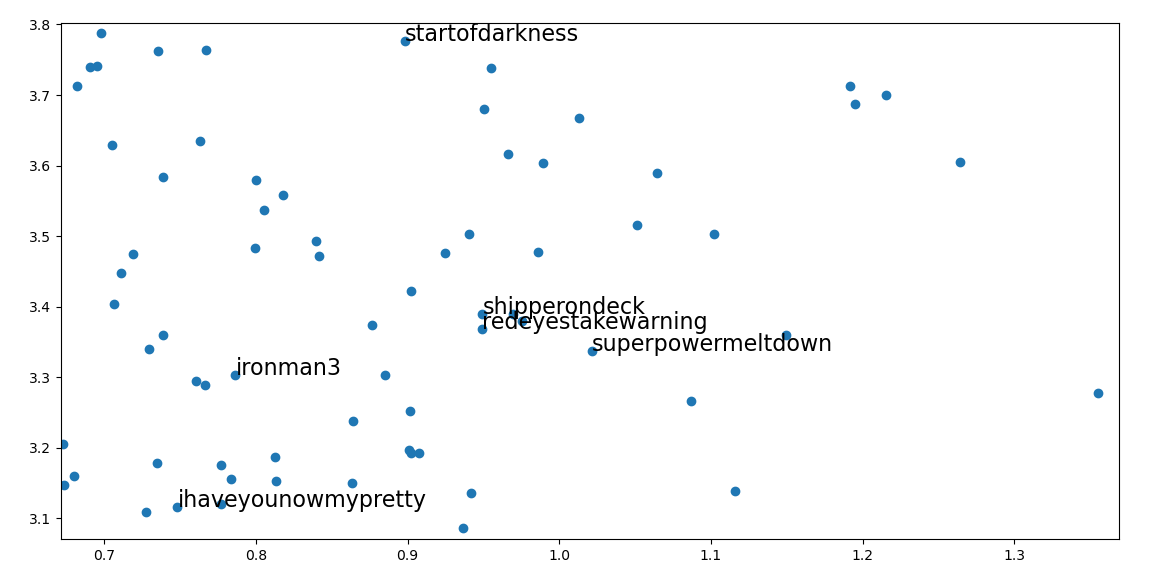
\includegraphics[width=1\linewidth]{../images/cluster-36-visualization-new-corpus-v3-1024-ironman3-font-16-zoom-in.png}
		\caption{Cluster visualization zoom in}
		\label{fig:cluster-visualization-zoom-in}
	\end{figure}
	
	
		\section{Results}
	\label{sec:res}
	
	\begin{figure}
		\centering
		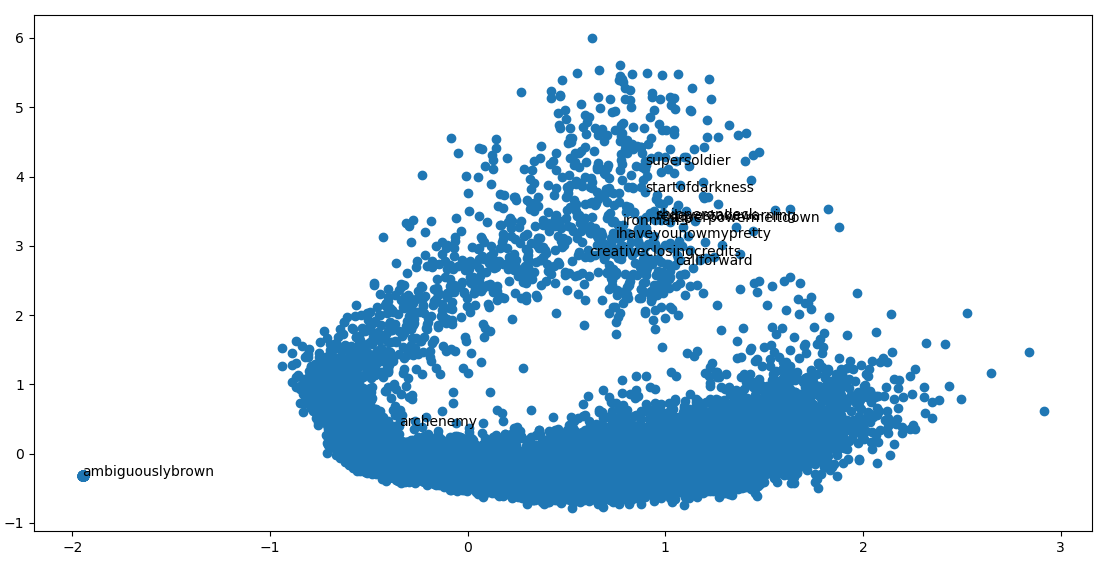
\includegraphics[width=1\linewidth]{../images/cluster-36-visualization-new-corpus-v3-1024-ironman3-zoom-out.png}
		\caption{Cluster visualization zoom out}
		\label{fig:cluster-visualization-zoom-out}
	\end{figure}
	
	
	
	\section{Conclusions, discussion and future work}
	 
	From the obtained results we can conclude that the fact of creating an artificial corpus improves the accuracy of the embedding vectors generated in relation to a natural language  corpus. The fact of being able to build the custom corpus allows us to avoid rhetorical elements derived from the use of natural language. In this way we can put the focus on the relationships between the entities and always put together those words that are related. We avoid so words that do not have a strong relationship appear close. 
	We have found two main difficulties when implementing this methodology:
	\begin{itemize}
	\item The first has been to find a metric that allows us to reinforce more important concepts. 
	\item Second one, has been to obtain a metric that allows us to evaluate the results.
    \end{itemize}
	It will be necessary to find these metrics in each problem where you want to apply this methodology
	
	Future work should focus on finding new ways to measure the accuracy of the results. In many cases finding relationships between entities is trivial when it comes to natural language. Clear examples of this can be the capitals of countries or find the feminine of some term. However, trying to achieve the same in areas where we are not very familiar can be much more complicated. Finding metrics that allow us to evaluate the accuracy of the model without the need to have a very deep knowledge of the work area would be an interesting future line of work. Another question worthy of being analyzed in future works, consists in finding characteristics in the real system that serve to reinforce with greater intensity those stronger relationships. In the dataset used we have used the popularity of films and tropes as a means of reinforcing more intensely the relationships between films and popular tropes. Better markers will allow the models to more accurately represent the relationships between the entities of the real system.
	
	
	% It is possible to create artificial corpus better than natural ones?
	
	% find other ways to build accuracy checklists 
	% Popular films will appear more times in corpus. This idea can be used to build the artificial corpus in future works.
	% Check if embedding vectors clusters can be used to obtain better accuracy check lists 
	\section{Acknowledgments}
	
	\bibliographystyle{iccc}
	\bibliography{iccc}
	
\end{document}
